\documentclass[a4paper,11pt, final]{report}
\usepackage{graphicx}
\usepackage{float}
\usepackage{url}
\usepackage{collcell}
\usepackage{caption}
\usepackage{multirow}
\usepackage{subcaption}
\usepackage[none]{hyphenat}
\usepackage{mathbbol}
\newcommand{\Lagr}{\mathcal{L}}
\newcommand{\includepic}[1]{\includegraphics[width=5cm,height=8cm,keepaspectratio]{#1}}
\newcolumntype{i}{@{\hspace{6ex}}>{\collectcell\includepic}c<{\endcollectcell}}
\usepackage{stackengine}
\def\delequal{\mathrel{\ensurestackMath{\stackon[1pt]{=}{\scriptstyle\Delta}}}}
\usepackage{algorithm}
\usepackage[noend]{algpseudocode}
\usepackage[none]{hyphenat}
\renewcommand\bibname{References}
\usepackage[utf8]{inputenc}
\usepackage{epsfig}
\usepackage{hyperref}
\usepackage{url}
\renewcommand\bibname{References}
\usepackage{color}
\usepackage{textcomp}
\usepackage{acronym}
\usepackage[top=0.5in, bottom=1in, left=1in, right=1in]{geometry}
\usepackage{xcolor}
\newcommand{\norm}[1]{\left\lVert#1\right\rVert}
\usepackage{sectsty}
\usepackage{comment}
\chapternumberfont{\large} 
\chaptertitlefont{\Huge}



\definecolor{dark-red}{rgb}{0.4,0.15,0.15}
\definecolor{dark-blue}{rgb}{0.15,0.15,0.4}
\definecolor{medium-blue}{rgb}{0,0,0.5}

\newcommand{\BigO}[1]{\ensuremath{\operatorname{O}\bigl(#1\bigr)}}
\parindent 8pt
\begin{document}
	\emergencystretch 3em
  \thispagestyle{empty}
  \vspace*{1cm}
  {\centering     
  \textbf{\LARGE Design and Development of Network Interface controller for AJIT processor based SoC}\\
  \vspace{1.20cm}
  \textbf{\large M.Tech Project Thesis}\\
  \vspace{1cm}
  {Submitted in partial fulfillment of the requirements}\\
  \vspace{0.25cm}
  {for the degree of}\\
  \vspace{1cm}
  \textbf{ Master of Technology}\\
  \textbf{Integrated Circuits and Systems}\\
  \vspace{1.50cm}
  {by}\\
  \vspace{0.20cm}
  \textbf{\large Mr. Harshad Bhausaheb Ugale}\\
  \vspace{0.25cm}
  \textbf{\large (Roll No. 20307R008)}\\
  \vspace{1.8cm}
  {Under the guidance of}\\
  \vspace{0.20cm}
  \textbf{\large Prof. Madhav P. Desai}\\
    \vspace{0.30cm}
  \vspace{1.450cm}
    \begin{figure}[htb]
    \begin{center}
    
\includegraphics[height=1.5in,width=1.5in]{logo.png}
    \end{center}
    \end{figure}

    
  {\textbf{Department of Electrical Engineering}}\\
  {\textbf{Indian Institute of Technology Bombay}}\\
  {\textbf{June 2023}}
 
 }
 

\newpage
\pagenumbering{roman}
 \linespread{1.5}
\chapter*{Declaration}
%\pagenumbering{gobble}
I declare that this written submission represents my ideas in my own words and where others ideas or words have been included, I have adequately cited and referenced the original sources. 
\newline
\newline
I also declare that I have adhered to all principles of academic honesty and integrity and have not misrepresented or fabricated or falsified any idea/data/fact/source in my submission. I understand that any violation of the above will be cause for disciplinary action by the Institute and can also evoke penal action from the sources which have thus not been  properly cited or from whom proper permission has not been taken when needed.

\vspace{3.0cm}
\begin{flushright}
\line(1,0){140}\\
\vspace*{10pt}
\textbf{Harshad Bhausaheb Ugale} \\
\textbf{Roll No. 20307R008} \\
IIT BOMBAY
\end{flushright}
\begin{flushleft}
%October, 2022

%14, June 2017.
Date: \today
%\line(1,0){75}
\end{flushleft}


 
 \newpage
\chapter*{Acknowledgements}
I wish to express my sincere gratitude to \textbf{Prof. Madhav P. Desai}, my supervisor for his valuable guidance and constant support.\\
I would also like to thank all the members of \textbf{VLSI Lab} for the continuous support throughout my work.\\
\\
\vspace*{0pt}
\begin{flushright}
\textbf{Harshad Bhausaheb Ugale}
\end{flushright}

\newpage

% \\\---------------------------------------------

\chapter*{Abstract} \addcontentsline{toc}{chapter}{Abstract}


\begin{comment}
	- Problem :
		
	- Highlight of work : One liner description, should include tools 
	- Results : latency, peak performance
	- Implication : How does this work add to the body of knowledge on the topic? Are there any practical or theoretical
			applications from your findings or implications for future research?
\end{comment}


The rapid advancement of network technologies has created a growing demand for efficient and reliable network communication solutions. As a result, the integration of a Network Interface Controller (NIC) into an indigenous AJIT processor-based System-on-Chip (SoC) has become increasingly crucial. This thesis aims to address this need by designing and developing a NIC that enables seamless network connectivity and communication capabilities for the AJIT processor. Additionally, it highlights the growing reliance of AI and ML technologies on network-based applications.

The outcomes of this research demonstrate the successful integration of the NIC into the AJIT SoC prototype. The NIC design and verification are carried out using AHIR-V2 tools, which provide an algorithmic approach to digital design. The developed NIC empowers the AJIT processor to efficiently send and receive data packets over the network, facilitating seamless connectivity with external devices and systems. Moreover, an AI/ML inference engine is employed to showcase the potential of leveraging Ethernet interface for advanced computational tasks.

The implications of this research extend beyond the immediate context of the AI/ML inference engine. The designed version of the NIC is flexible and can be modified to incorporate additional complex functionalities, such as self-routing and NIC-to-NIC communication. This opens up possibilities for the development of routers and other network devices with multiple NICs, offering enhanced network capabilities.
%This thesis focuses on the design and development of a network interface for the AJIT processor, an indigenous high-performance processor. The objective was to enhance the processor's functionality by incorporating an Ethernet interface. A network interface design was proposed and implemented, including hardware components, software drivers, and firmware. Extensive testing demonstrated successful integration, showcasing good performance and robustness. This research expands the capabilities of the AJIT processor, making it a more versatile platform for networked computing applications such as router.


\tableofcontents
  \addcontentsline{toc}{chapter}{\listfigurename}
  \listoffigures
%  \printglossaries
  \listoftables

  
  
%---------------------------------------------------------------------------
%--------- CHAPTER 1 - Introduction
%---------------------------------------------------------------------------
\begin{comment}
	Context -: Do setting for gurther reading

	Goals

	Challenges
\end{comment}
\chapter{Introduction}
\pagenumbering{arabic}

The rapid advancement of network technologies has revolutionized various aspects of our lives, ranging from communication to data processing and beyond. In this era of interconnected systems, the need for efficient and reliable network communication solutions has become paramount. The integration of a Network Interface Controller (NIC) into an indigenous AJIT processor-based System-on-Chip (SoC) serves as a crucial step towards achieving seamless network connectivity and communication capabilities.

This chapter provides an introduction to the design and development of a Network Interface Controller for the AJIT processor-based SoC. The AJIT processor, being an indigenous processor, offers unique opportunities for customization and optimization to meet specific requirements. By integrating a NIC, the AJIT SoC can effectively send and receive data packets over the network, enabling seamless connectivity with external devices and systems. Furthermore, this chapter discusses the goals and challenges, associated with the design and development of the Network Interface Controller. The goals include integrating the Ethernet interface into the AJIT SoC prototype, demonstrating the use of an AI/ML acceleration application, and generalizing the design for network appliance SoCs such as routers. By achieving these goals, the research contributes to the broader field of network communication solutions. 

Overall, this chapter sets the stage for the subsequent chapters, which delve into the design, implementation, and evaluation of the Network Interface Controller. It establishes the importance of network connectivity in the context of the AJIT processor-based SoC and provides a roadmap for the rest of the thesis



	\section{Goals}

		\subsection{Integration of Ethernet into AJIT System-on-Chip (SoC) Prototype}
			The first goal is to successfully integrate an Ethernet interface into the AJIT SoC prototype. This involves designing and implementing the necessary hardware components(Network Interface Controller) and firmware to enable Ethernet connectivity.

		\subsection{Network-Accelerated AI/ML Application using Ethernet Interface}
			The second goal is to utilize the integrated Ethernet interface of the AJIT processor to enable network-accelerated execution of AI/ML accleration application. This demonstration highlights the synergy between the processor's advanced computing capabilities and the enhanced connectivity, showcasing the seamless integration of the Ethernet interface to support efficient processing and communication in networked AI/ML workloads.

		\subsection{Generalization to Network Appliance SoC (Router)}
			The third goal aims to generalize the network interface design to a broader context by extending it to a network appliance SoC, specifically a router. This involves evaluating the feasibility of incorporating the network interface into a router SoC, considering factors such as performance, power consumption, and compatibility with networking protocols.

By achieving these goals, this research aims to enhance the AJIT processor's capabilities and explore its potential in networked computing systems, paving the way for future advancements in indigenous processor development.

	\section{Challenges}

		\subsection{Network Interface Controller Design and Validation}
   One of the key challenges in this research is the design and validation of the network interface controller. This involves designing a controller that can efficiently handle the transmission and reception of Ethernet packets, ensuring proper synchronization, error handling, and protocol compliance. The validation process includes rigorous testing to verify the functionality, performance, and reliability of the controller under different network conditions and workloads.\\

		\subsection{Integration of Xilinx's MAC IP}
   Another challenge is the integration and configuration of Xilinx's MAC (Media Access Controller) IP into the network interface design. This requires understanding the specifications and functionality of the MAC IP and ensuring its seamless integration with the AJIT processor's architecture. The challenge includes addressing any compatibility issues, optimizing configurations, and verifying the correct operation of the MAC IP within the overall network interface design.\\

		\subsection{Software Design for Reliable Exchange of Information over Ethernet}
   Implementing reliable communication over Ethernet presents a challenge that requires careful software design. This involves developing protocols and algorithms to ensure the reliable exchange of information between the AJIT processor and external devices connected via Ethernet. The software design should handle packet loss, retransmissions, flow control, and other mechanisms to guarantee the integrity and timeliness of data transmission in the networked environment.\\

		\subsection{Software Design for SOC Firmware in AI/ML Acceleration Application}
   In the context of the AI/ML acceleration application, a significant challenge lies in the software design of the system-on-chip (SoC) firmware. This involves developing firmware that efficiently interacts with the network interface, handles data transmission and reception, and interfaces with the AI/ML acceleration modules. The firmware should be optimized for performance, ensuring seamless integration of the AI/ML application with the Ethernet interface and leveraging the network acceleration capabilities of the AJIT processor.\\



%---------------------------------------------------------------------------
%--------- CHAPTER 2 - Design and Validation of Network Interface Controller
%---------------------------------------------------------------------------
\chapter{Design and Validation of Network Interface Controller}

This chapter focuses on the design and validation of the Network Interface Controller (NIC) for the AJIT processor-based System-on-Chip (SoC). The NIC plays a critical role in enabling network connectivity and communication capabilities within the SoC.

The design of the NIC involves several components and considerations, including the network protocol support, data packet handling, memory management, and interface with the AJIT processor. To ensure a robust and reliable design, the NIC undergoes a rigorous validation process to verify its functionality, performance, and compatibility with the AJIT SoC architecture.

The primary goal of this chapter is to provide a detailed overview of the design process, highlighting the key components and their interconnections. It explores the challenges encountered during the design phase and discusses the solutions and design choices made to overcome them. Additionally, the chapter delves into the validation methodologies employed to ensure the correctness and efficiency of the NIC design.

By describing the design and validation of the NIC, this chapter aims to provide insights of implementing a network interface solution for the AJIT processor-based SoC. It serves as a foundation for subsequent chapters, which will explore specific aspects of the NIC design, such as the data packet handling mechanisms, and memory management schemes.

	
	\section{Design decisions}
		Before directly jumping on NIC design lets take a look at necessry design decisions made. The NIC will receive packet data from MAC
		which will be stored in memory. Processor will need to allocate this memory and provide that information to NIC. This overall needs to
		3 main interfaces to NIC. The figure~\ref{fig:NIC-Proc-top-level} shows all the interfaces. Lets see each interface in detail.	

		\begin{figure}[h]
			\centering
			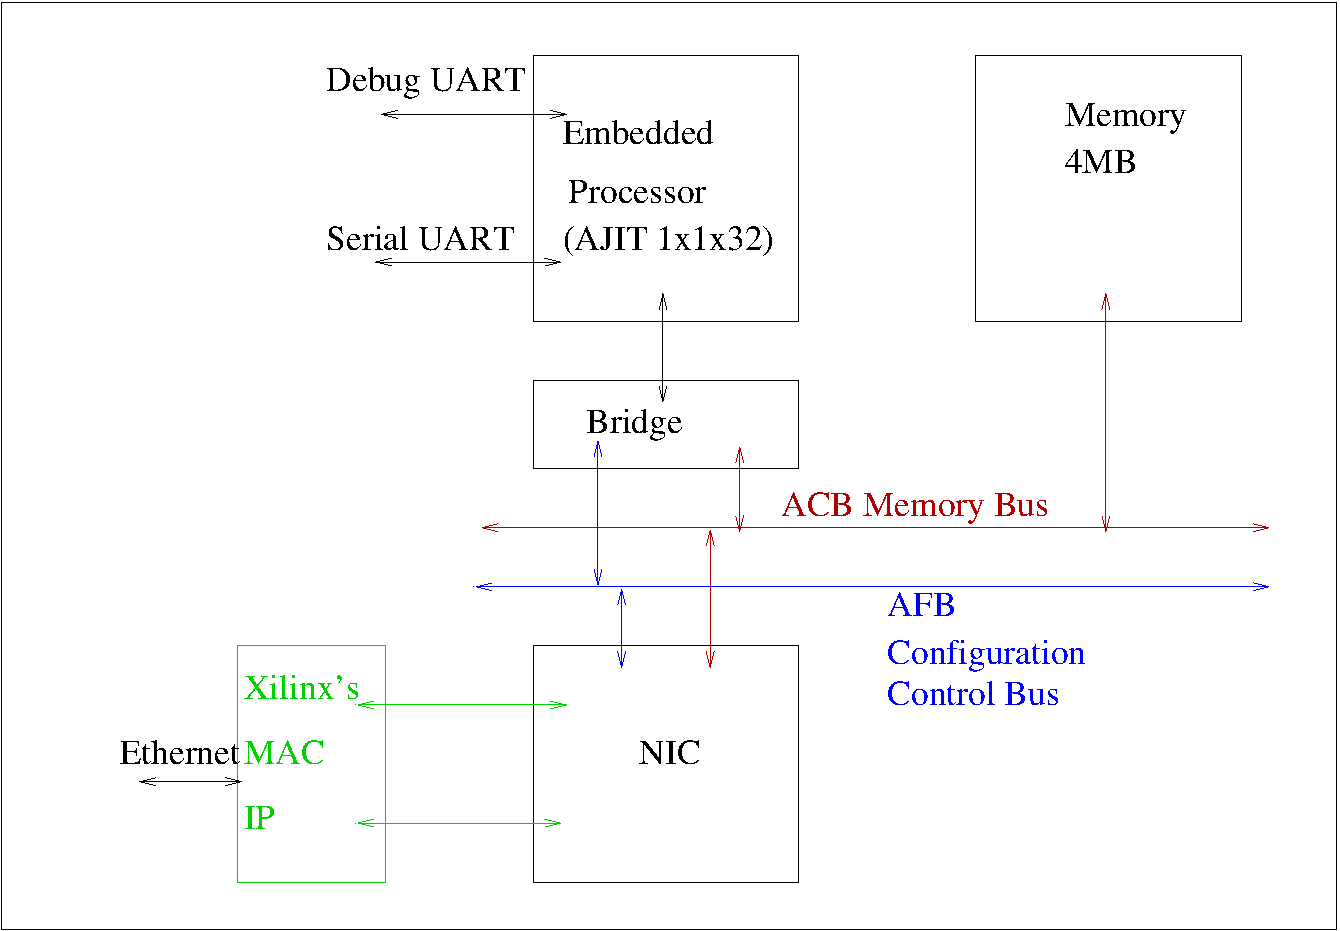
\includegraphics[width=10cm]{./figures/top_level_for_interfaces.pdf}
			\caption{Top level with Interfaces}
			\label{fig:NIC-Proc-top-level}
		\end{figure}




		\subsection{NIC-MAC interfce}
			NIC to MAC interface will used by NIC for receiving and transmitting packtes from MAC. The memory which will be used is provides 8 bytes per request.
			so this interface is kept 73(64 bit data + 9 bit control) bits. The bit mapping is as shown in table~\ref{tab:NIC-MAC-interface}.
				\begin{table}[!htbp]
					\centering
					\begin{tabular}{ccl}
						\hline
						\textbf{Signal Name} & \textbf{Location} &\textbf{Signal Description}  \\ \hline
						\multirow{2}{*}{\textit{tlast}}	& \multirow{2}{*}{[72:72]}	& \textit{tlast} becomes `1' if the 64 bit chunk is last\\
										& 				& chunk of packet.\\ \hline
						\textit{tdata}   		& [71: 8] 			& \textit{tdata} is actual packet data chunk\\ \hline
						\multirow{3}{*}{\textit{tkeep}}	& \multirow{3}{*}{[ 7: 0]}	& \textit{tkeep} is 8 bit field, each bit is mapped\\
										&				& to 8 bytes of data. if any bit is `1' then\\
										& 				& corresponding byte in data is valid else not.\\ \hline 
					\end{tabular}
					\caption{NIC-MAC interface description}
					\label{tab:NIC-MAC-interface}
				\end{table}
			Same interface will be used for both reception and transmission of packet.

		\subsection{NIC-Memory interface}
			NIC-Memory interface is required for store and load of packets to and from memory. Already developed ACB(AJIT Core Bus) protocol will be used for this.
			The protocol consists of two interfaces,
			\begin{enumerate}
				\item ACB Requeuest : Requests from NIC to store and load the packet will be sent through this interface. see~\ref{tab:NIC-Memory-interface-req} for bit mapping.
				\item ACB Response : Response generated by memory to the request will be sent back to NIC on this interface. see~\ref{tab:Memory-NIC-interface-resp} for bit mapping.
			\end{enumerate}

				\begin{table}[!htbp]
					\centering
					\begin{tabular}{ccl}
						\hline
						\textbf{Signal Name} 			& \textbf{Location} 		&{c}\textbf{Signal Description}  \\ \hline
						\multirow{2}{*}{\textit{lock}}		& \multirow{2}{*}{[109:109]}	& lock bit, if set to `1' by a master then\\
											&				& other master's don't get access to Mmory.\\ \hline
						\multirow{2}{*}{\textit{read/write\_bar}}& \multirow{2}{*}{[108:108]}	& if `1', the request is read request,\\ 
											& 				& if `0', the request is write request.\\ \hline
						\multirow{3}{*}{\textit{byte\_mask}}	& \multirow{3}{*}{[ 107: 100]}	& \textit{byte\_mask} is 8 bit field, each bit is mapped\\
											&				& to 8 bytes of data. if any bit is `1' then\\
											& 				& corresponding byte in data is valid else not.\\ \hline 
						\multirow{2}{*}{\textit{address}}   	& \multirow{2}{*}{[99:64]} 	& addres(byte) where read/write should\\ 
											&				& be performed.\\ \hline
						\textit{write\_data}   			& [63: 0] 			& Data to be written.\\ \hline
					\end{tabular}
					\caption{NIC - Memory interface description}
					\label{tab:NIC-Memory-interface-req}
				\end{table}

				\begin{table}[!htbp]
					\centering
					\begin{tabular}{ccl}
						\hline
						\textbf{Signal Name} 		& \textbf{Location} 		&\textbf{Signal Description}  \\ \hline
						\textit{err}			& [64:64]			& Value `1' indicates errored response.\\\hline
						\textit{data}   		& [63: 0] 			& Contains read data if the req. was read req.\\ \hline
					\end{tabular}
					\caption{Memory - NIC interface description}
					\label{tab:Memory-NIC-interface-resp}
				\end{table}
			
		\subsection{NIC-Processor interface}
			This will be more of a control interface. Processor will allocate the memory space for packet storage and provide thaat info to NIC using this interface.
			NIC will have registers inside which will written by processor using this interface. For further information see~\ref{subsec:NIC_reg}. An already developed
			AFB(AJIT FIFO Bus) protocol will be used for this. This AFB protocol also has two interfaces like ACB protocol only the address width is half.

			\begin{enumerate}
				\item AFB Requeuest : Requests from Processor to write or read the NIC reg will be sent through this interface. see~\ref{tab:Proc-NIC-interface-req} for bit mapping.
				\item AFB Response : Response generated by NIC to the request will be sent back to Processor on this interface. see~\ref{tab:NIC-Proc-interface-resp} for bit mapping.
			\end{enumerate}

				\begin{table}[!htbp]
					\centering
					\begin{tabular}{ccl}
						\hline
						\textbf{Signal Name} 			& \textbf{Location} 		&{c}\textbf{Signal Description}  \\ \hline
						\multirow{2}{*}{\textit{lock}}		& \multirow{2}{*}{[73:73]}	& lock bit, if set to `1' by a master then\\
											&				& other master's don't get access to Mmory.\\ \hline
						\multirow{2}{*}{\textit{read/write\_bar}}& \multirow{2}{*}{[72:72]}	& if `1', the request is read request,\\ 
											& 				& if `0', the request is write request.\\ \hline
						\multirow{3}{*}{\textit{byte\_mask}}	& \multirow{3}{*}{[ 71: 68]}	& \textit{byte\_mask} is 4 bit field, each bit is mapped\\
											&				& to 4 bytes of data. if any bit is `1' then\\
											& 				& corresponding byte in data is valid else not.\\ \hline 
						\multirow{2}{*}{\textit{address}}   	& \multirow{2}{*}{[67:32]} 	& addres(byte) where read/write should\\ 
											&				& be performed.\\ \hline
						\textit{write\_data}   			& [31: 0] 			& Data to be written.\\ \hline
					\end{tabular}
					\caption{Processor - NIC interface description}
					\label{tab:Proc-NIC-interface-req}
				\end{table}

				\begin{table}[!htbp]
					\centering
					\begin{tabular}{ccl}
						\hline
						\textbf{Signal Name} 		& \textbf{Location} 		&\textbf{Signal Description}  \\ \hline
						\textit{err}			& [32:32]			& Value `1' indicates errored response.\\\hline
						\textit{data}   		& [31: 0] 			& Contains read data if the req. was read req.\\ \hline
					\end{tabular}
					\caption{ NIC - Procesor interface description}
					\label{tab:NIC-Proc-interface-resp}
				\end{table}

	
	\section{Interfaces data structures}

		The interface data structures used in the NIC design consist of three queues: the free\_queue, rx\_queue, and tx\_queue.


		\begin{comment}
		\begin{figure}[h]
			\centering
			\includegraphics[width=8cm]{./figures/queues.pdf}
			\caption{Add this fig which will have all queue interfaces}
			\label{fig:queue_interface}
		\end{figure}
		\end{comment}


	\begin{itemize}
		\item \textbf{free\_queue}: This queue holds the addresses of free buffers that are available for storing packets. The processor initially assigns a set of buffers and pushes their addresses into the free\_queue. These buffers do not have any active packets and are ready to be utilized for storing incoming packets. Both the processor and the NIC can push and pop from the free\_queue.\\

		\item \textbf{rx\_queue}: The rx\_queue is pushed by the NIC and popped by the processor. It holds the addresses of buffers that currently contain active packets. When the NIC receives a packet, it stores the packet in a buffer and pushes the address of that buffer into the rx\_queue. This allows the processor to identify the buffers with active packets that are ready for processing.

		\item \textbf{tx\_queue}: The tx\_queue is pushed by the processor and popped by the NIC. Once the processor has finished processing a packet, it pushes the address of the processed packet buffer into the tx\_queue. The NIC monitors the tx\_queue and retrieves the buffer addresses from it to send the packets out over the network.\\
	\end{itemize}

These queues enable efficient coordination and communication between the processor and the NIC, ensuring the proper handling and processing of packets.The queue header format is shown below,
		\begin{verbatim}
		typedef struct _CortosQueueHeader {
		        uint32_t totalMsgs; // current total messages
		        uint32_t readIndex;
		        uint32_t writeIndex;
		        uint32_t length;
		        uint32_t msgSizeInBytes;
		        uint8_t *lock;
		        uint8_t *bget_addr;
		        // if misc == 1, then assume single writer 
		        // and single reader and don't use locks
		        uint32_t misc;
		} CortosQueueHeader;
		\end{verbatim}
	

To ensure synchronization and prevent conflicts during access to these queues, a locking mechanism is implemented. The locking mechanism utilizes atomic operations, which guarantee thread-safe access and modifications to the queues. This ensures that only one entity can perform push and pop operations on the queues at a given time, preventing simultaneous modifications and preserving the integrity of the queue data.


At startup, the processor initializes the queues by allocating memory for them and configuring their initial state. The addresses of these queues are then communicated to the NIC by writing to specific NIC registers. This process allows the NIC to access and manipulate the queues effectively during runtime. Let's see the NIC registers now.


		These are all interface decisions taken lets now move on to NIC design.
	\section{Network Interface Controller}
		

		\begin{figure}[h]
			\centering
			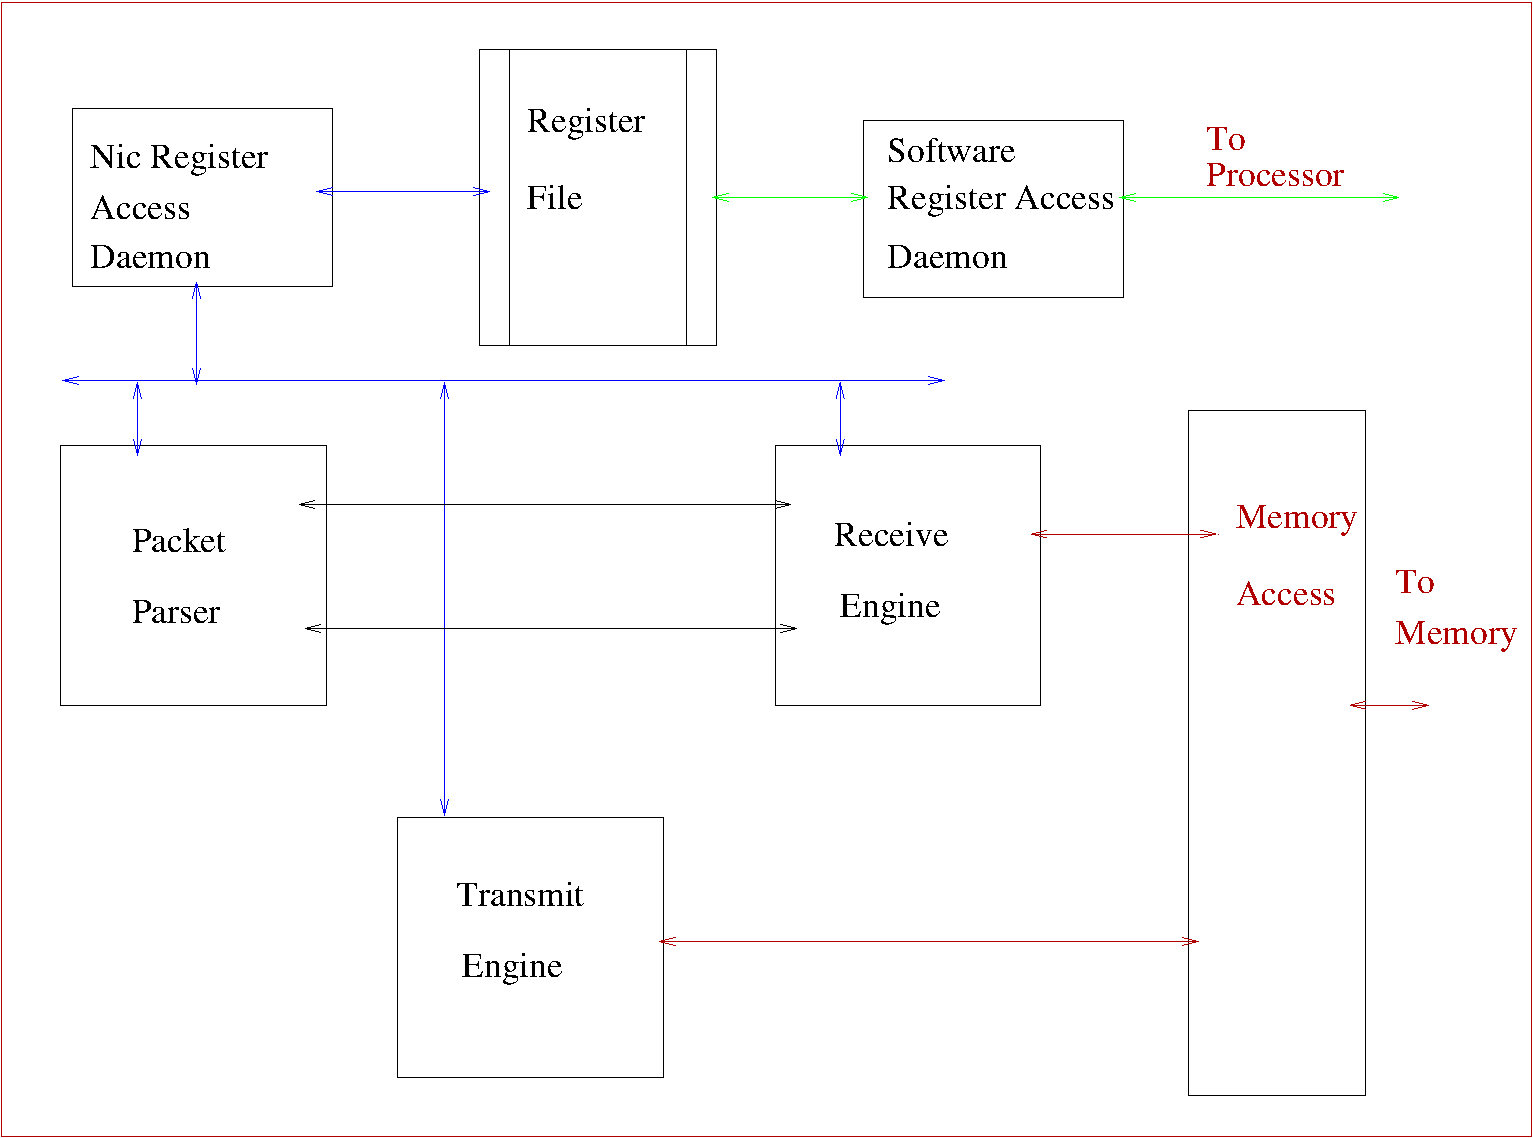
\includegraphics[width=10cm]{./figures/NIC_Internal.pdf}
			\caption{Architecture of Network Interface Controller}
			\label{fig:NIC-Arch}
		\end{figure}

		\subsection{Register File Map}
				The NIC (Network Interface Controller) registers are specific memory locations within the NIC that are used for configuration, control, and status monitoring purposes. These registers allow communication between the processor and the NIC, enabling the processor to control and monitor NIC. The NIC registers provide a standardized interface for the processor to interact with the NIC and perform tasks such as enabling or disabling the NIC, setting queue address and monitoring the status of data transmission and reception.

			\begin{table}[htbp]
				\centering
				\begin{tabular}{|c|c|c|}
					\hline
					Reg. ID& Address offset & Description  \\ \hline
					0  & 0x00  & Control reg    \\ \hline
					1  & 0x04  & Number of Servers    \\ \hline
					2  & 0x08  & Address of rx\_queue    \\ \hline
					10  & 0x28  & Address of tx\_queue    \\ \hline
					18  & 0x48  & Address of free queue    \\ \hline
				\end{tabular}
				\caption{NIC registers map}
				\label{tab:NIC_REG}
			\end{table}

		\subsection{Packet Storage Format}

		\subsection{Parser}
				The parser daemon, receives data from the MAC (Media Access Control) through a pipe and extracts relevant information from Ethernet packets. It utilizes a state machine to process chunks of data and identifies essential details such as source and destination MAC addresses, type/length field, and packet data. The parsed information is then forwarded to receve engine daemon.
		\begin{verbatim}
			loop1 :
			if(enable_by_processor)
			       loop2 :
			       -> read from MAC
			       -> if(Header) 
			                -> send to header & packet pipe
			                -> goto loop2
			       -> else
			       	        -> send to packet pipe
			       	        -> goto loop2
			else
			       -> goto loop1
		\end{verbatim}

		\subsection{Receive Enigne}
				The receive engine daemon is responsible for storage of packets coming from parser. It receives the parsed packet information from the parser daemon and interacts with the processor to ensure the proper handling of received packets. The receive engine daemon uses the free\_queue, to get empty buffer address tp store the active packets in buffers.
			Then uses rx\_queue to provide their(buffer's) addresses to the processor for processing. The algorith of receive engine is shown below,
		\begin{verbatim}
			loop1 :
			if(enable_by_processor)
			       loop2 :
			       -> count = 0;
			       -> buf_addr = pop from free queue
			       loop2.1:
			       -> Read from header_pipe and write to buff_addr
			       -> count++
			       -> if(!header_end)
			       	        -> goto loop2.1
			       loop2.2:
			       -> Read from packet pipe and write to buf_addr 
			       -> count++
			       -> if(last_chunk)
			       	        -> write count and last bytemast to buf_addr[0].
			       	        -> push buf_addr to rx_queue.
			                -> goto loop2
			       -> else
			       	        -> goto loop2.2
			else
			       -> goto loop1
		\end{verbatim}

		\subsection{Transmit Engine}
				The transmit engine daemon focuses on transmitting processed packets from the processor to the external network. It receives the addresses of processed packet buffers from the processor via the tx\_queue and sends the corresponding packets out through the Ethernet interface. The transmit engine daemon monitors the tx\_queue and retrieves the buffer addresses to facilitate efficient packet transmission. The daemon also pushes free\_queue with the address of buffer which is sent out. This allows resue of buffers. The algorith of transmit engine is shown below,
		\begin{verbatim}
			loop1 : 
			if(enable_by_processor)
			        loop2:
			        -> buf_addr = try to pop tx_queue
			        -> if(pop successful)
			                -> Rx = read control data(buf_addr[0]) 
			                -> count = extractCountFromRx(Rx)
			                loop3:
			                -> read packet from buf_addr
			                -> send out to MAC
			                -> count--
			                -> if(count == 0)
			                        -> push buf_addr to free_queue.
			                        -> goto loop2 
			                -> else
			                        -> goto loop3
			        -> else
			                        -> goto loop2
			->else
			        goto loop1
		\end{verbatim}

		\subsection{Software register Access}
				The software register access daemon enables the processor to access and modify the NIC's software registers. These registers contain various control and configuration parameters, allowing the processor to configure and manage the behavior of the NIC. The software register access daemon handles the communication between the processor and the NIC registers, ensuring reliable and secure access. Processor uses AFB protocol(see ~\ref{AFB}) for register access.\\

	

		\subsection{Nic register Access}
				The NIC register access daemon provides the necessary interface for the NIC to read from and write to its internal registers. These registers store critical information for the proper functioning of the NIC, including configuration settings, status flags, and other control parameters. The NIC register access daemon ensures that the processor can interact with these registers and modify them as needed to configure and manage the NIC's behavior.\\
		\begin{table}[!htbp]
					\centering
					\begin{tabular}{ccl}
						\hline
						\textbf{Signal Name} 			& \textbf{Location} 		&{c}\textbf{Signal Description}  \\ \hline
						\multirow{2}{*}{\textit{read/write\_bar}}& \multirow{2}{*}{[42:42]}	& if `1', the request is read request,\\ 
											& 				& if `0', the request is write request.\\ \hline
						\multirow{3}{*}{\textit{byte\_mask}}	& \multirow{3}{*}{[ 41: 38]}	& \textit{byte\_mask} is 4 bit field, each bit is mapped\\
											&				& to 4 bytes of data. if any bit is `1' then\\
											& 				& corresponding byte in data is valid else not.\\ \hline 
						\multirow{2}{*}{\textit{reg\_index}}   	& \multirow{2}{*}{[37:32]} 	& index of register to which read/write should\\ 
											&				& be performed.\\ \hline
						\textit{write\_data}   			& [31: 0] 			& Data to be written.\\ \hline
					\end{tabular}
					\caption{NIC to Ref file interface description}
					\label{tab:NIC-Reg-interface-req}
				\end{table}

				\begin{table}[!htbp]
					\centering
					\begin{tabular}{ccl}
						\hline
						\textbf{Signal Name} 		& \textbf{Location} 		&\textbf{Signal Description}  \\ \hline
						\textit{err}			& [32:32]			& Value `1' indicates errored response.\\\hline
						\textit{data}   		& [31: 0] 			& Contains read data if the req. was read req.\\ \hline
					\end{tabular}
					\caption{ Reg file to NIC interface description}
					\label{tab:Reg-NIC-interface-resp}
				\end{table}


		\section{Main helper modules}
			\begin{enumerate}
				\item \textbf{memoryAccess}: \\
				\item \textbf{pusiIntoQueue}: \\
				\item \textbf{popFromQueue}: \\
				\item \textbf{acquireLock}: \\
				\item \textbf{releaseLock}: \\
			\end{enumerate}	
	\section{NIC and Processor Integration}
	
	\section{Validation and Performance}
		The data rate found using 1x1x32 (single core single threaded) AJIT processor are as shown in table~\ref{table_dataRate}
		\begin{table*}[h!]
			\caption{Data rate achieved for differnet number of packets \& packet sizes}
			\begin{center}
				\begin{tabular}{|c|c|c|c|}
					\hline
					& \multicolumn{3}{c|}{\textbf{Packet Size}(in Bytes)}\\
					\hline
					\textbf{No. of Packets}& \textbf{48}			& \textbf{136}			& \textbf{236} 	  \\
					\hline
					&  \multicolumn{3}{c|}{\textbf{Data Rate}(in Mbps)}\\	
					\hline
					1			& 11.3316		  	& 31.7085			& 51.2869 \\
					\hline
					10			& 18.8431		  	& 57.2255			& 102.4069\\
					\hline
					100			& 22.4589		  	& 64.1140			& 110.9845\\
					\hline
					500			& 22.9792		  	& 64.0819			& 114.2853\\
					\hline
					1000			& 23.0982			& 64.0665			& 114.4293\\
					\hline
					5000			& 23.0336			& 64.3663			& 114.7432\\
					\hline
					10000			& 23.0892			& 64.3163			& 114.7907\\
					\hline
					50000			& 23.0983			& 64.4662			& 114.8123\\
					\hline
				\end{tabular}
				\label{table_dataRate}
			\end{center}
		\end{table*}
	
	Only NIC with Memory we are able to achieve 433.2847 Mbps for 1750 packets of size 146 Byets.


\begin{comment}
	Brief Context 
		System information top level diagram its desrciption 
		- Interfaces
			- NIC - Proc
			- NIC - MAC
			- NIC - Memory
	1. Network Interface Controller design
		2-3 statements related to it explaining functionality
		- all 5 Daemons
		- all helper modules
		- register file desription
		- Packet storage format
		NIC Can be modified further

	2. NIC-Processor Integration
		- NIC as MMIO
		- 
	3. Validation
		2-3 statements for setting
		- test setup
		- performance

	Driver for HOST and Software for AJIT processor were also written for same which will be discussed in next chapter.
\end{comment}



%---------------------------------------------------------------------------
%--------- CHAPTER 3 - SOC Design and Validation
%---------------------------------------------------------------------------
\begin{comment}
	Brief context
	1. proc - accl - NIC integration
	
	2. Driver for HOST

	3. Software for AJIT processor

	4. Validation
		2-3 statements
		- test setup
		- Performance
\end{comment}
\chapter{SoC Design and Validation}
We validate an characterize the perofrmance of the accelerator by integrating it into a System-on-chip (SoC) using AJIT Processor, which provides the accelerator with the commands to operate, and reads back the data. The whole system is also connected to a Network Interface Card, which provides high-speed IO for quick loading of images into the memory. The architecture of the system is shown in Fig~\ref{fig:SoC}.
\\

The system consists of 32bit wide AJIT processor at its core. The processor has an ACB interface through which it interacts with memory and other modules. The AFB interface linked to the Network Interface Controller (NIC) and the 8-engine acclerator cluster is used to transfer configuration information from the processor and relay back status flags to it. The modules are also provided with an ACB interface through which they can access the memory. The memory subsystem consists of a DRAM controller connected to an ACB to UI conversion protocol, which translates memory requests in the ACB bus to DRAM requests, and vice versa for the responses. In addition to the above, the processor has a couple of UART interfaces with which it can communicate with the outside world. Also, the NIC has an interface to connect with the Xilinx MAC IP, using which it can communicate to the host machine via Ethernet, currently configured to run at 100Mbps. 
\\
		\begin{figure}[h]
			\centering
			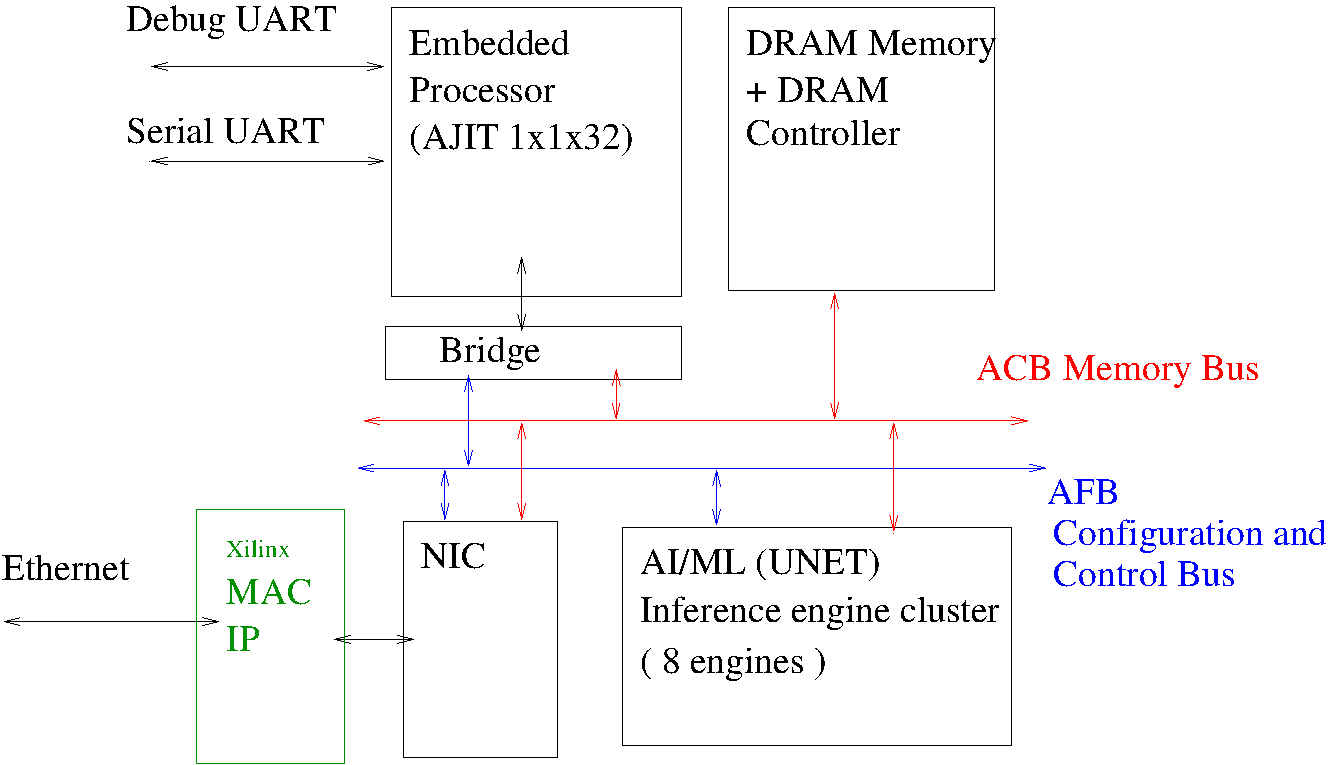
\includegraphics[width=12cm]{./figures/BlockDiagram.pdf}
			\caption{NIC, Processor and accelerator Soc Design}
			\label{fig:SoC}
		\end{figure}

		\clearpage
The pseudocode for the processors code is as follows:

\begin{verbatim}[numbers=left]
initialiseMemorySpaces()
initialiseNicQueues()
fetchKernelsThroughEthernet()

while(1) do
	fetchInputsThroughEthernet()
	
	initliaseAcceleratorStates()
	
	while (all accelerators not done) do
		for engine in list_of_engines do
			convolve(engine,stage)
			updateState(engine,stage)
		end for
	end while
	sendOutputsThroughEthernet()
end while
\end{verbatim}

The above pseudocode explains the working of the processor code. It first initialise memory spaces required by all modules. These include the queues required by NIC, the kernel addresses for the accelerators and the memory spaces for receiving and storing tensors during computation by the engines. After the memory spaces are initialised, all the queues for NIC are configured and initialised, and the Network Interface Controller starts executing. The kernels are then fetched in through Ethernet, which is then followed by the input tensors for all the engines. With the setup ready, NIC is turned off and the engines are allowed to execute on the data stage by stage. When all the acclerators are done with their computation, the output data is sent to the host PC through Ethernet, where the output is verified for correctness.
\\

The above is a simplified driver to demonstrate the functionality of using multiple accelerator engines inside the system using polling. The processor and the  accelerators both support the use of interrupts. The Interrupt Service Routine corresponding to the accelerator interrupts can be suitably confiured to allow the processor to be used for other processes, while the engines work on the compute-intensive AI/ML tasks, the completion of which can be signalled to the processor, at which the processor interrupts and schedules the next task to the accelerator before resuming its own execution.
\\


\section{Processor NIC Interface}

The processor initialises the queues for the NIC and starts the NIC. When NIC recives data from MAC it pops the free\_queue which has empty packet buffers address stored in it and writes the packet to that buffer. After successfully writting the packet NIC pushes the address of buffer to rx\_queue, any buffer address in rx\_queue indicates that this is the received packet and needs some action by processor. While this thing is going on processor keeps polling the rx\_queue, as soon as it gets any data over there it reads it and takes decision. In this setup processor is expected to store the packet at some memory location which is shared with acclerator through its registers. After this packet storage is complete processor pushes this address to tx\_queue which works as acknowledgement for the host, after receiving which it(host) sends new packet. This is overall flow for storing file in the memroy.
\\

Now to send file out on ethernet interface processor breaks file into number of packets, pops free\_queue for empty buffer address and stores packet at that address. After storing packet successfully processor pushes the buffer address to tx\_queue. The transmit engine running inside NIC which is polling this tx\_queue reads that buffer and sends it out. One by one all the packets sent out.



\section{Processor Accelerator Interface}

The processor begins by feeding the data to the registers 1 to 12. After that, it sets the bits 0 and 2 of register 0, which signals the accelerator to start working. The processor can then continue with other tasks or poll on the register 0 as it waits for the accelerator to complete, which is indicated by setting bit 4 of register 0 as high. Then, the processor updates the registers to the parameters for the next stage or image.
\\

In addition, the accelerator has a control daemon which resets the registers, reads the data from the AFB\_ACCELERATOR\_REQUEST, writes them onto the accelerator registers, and sends back the resposne to the AFB\_ACCELERATOR\_RESPONSE. The control daemon runs infinitely waiting on AFB\_ACCELERATOR\_REQUEST requests from the processor.
\\

The accelerator also has a worker daemon, which waits for the appropriate bits to be set in the r0 register. When the processor sends the request to execute through the registers, it calls the core function with the parameters stored by the processor in other registers. When the execution is completed, it writes back 0 into bit 4 of r0, thereby signalling the processor that the computation is completed.
\\

The accelerator also has an interrupt daemon which waits on bit 4 of r0, and sets the signal ACCELERATOR\_INTERRUPT\_8 corresponding to the above bit. The interrupt signal is not currently used, but can be utilised to prevent the processor from polling on r0 while the accelerator performs the computation.
\\


\section{Scaling The Number Of Engines}\label{sec:scale_eng}

In \ref{ch:3}, we described how the engine can eploit parallelism to obtain higher throughput. In this section, we characterize the throughput improvement obtained by exploiting the parallelism between different images by implementing multiple accelerator engines in a single cluster, each working on its own input image. The number of engines actively running were increased from one to eight, and the following results were obtained:
\\
\begin{comment}
\begin{table}
	\resizebox{\textwidth}{!}
	{
		\centering

		\begin{tabular}{P{0.16\linewidth} P{0.22\linewidth} P{0.22\linewidth} P{0.16\linewidth} P{0.16\linewidth}}
		\toprule
			No. of active cores & 	Total time taken (in clock cycles)  &	Time per image (*$10^6$ clock cycles)	& Utilisation (normalised with one engine)  & Speedup (normalised with one engine)\\
\toprule
1 & 93,249,712  & 93.25 & 1 & 1\\
\midrule
2 & 95,992,518  & 48.00 & 0.97 & 1.94\\
\midrule
3 & 99,271,600  & 33.09 & 0.94 & 2.82\\
\midrule
4 & 106,323,270  & 26.58 & 0.87 & 3.48\\
\midrule
5 & 116,061,718  & 23.21 & 0.80 & 4.00\\
\midrule
6 & 129,573,610  & 21.59 & 0.72 & 4.32\\
\midrule
7 & 144,883,176  & 20.69 & 0.64 & 4.47\\
\midrule
8 & 159,762,229  & 19.97 & 0.58 & 4.64\\
		\bottomrule
		\end{tabular}
	}
	\caption{Characterization of the performance of inference engine cluster}
	\label{tab:scale}
\end{table}
\end{comment}
From the data, it is evident that we can effeciently scale the system to support 4 accelerator engines running in parallel without significant loss of performance. The performance degradation stems primarily from the use of shared ACB connection to the memory, thereby causing contention for the resource. The degradation is small for upto 5 accelerators because the memory is being utilised around 10\% of the time, as seen in Table~\ref{tab:stage}. However, beyond 5 systems, the link becomes the bottleneck leading to greater performance degradation.
\\

The primary reason for the degradation is the use of limited memory bandwidth, which is being multiplexed by all the engines.







%---------------------------------------------------------------------------
%--------- CHAPTER 4 - Summary
%---------------------------------------------------------------------------
\begin{comment}
	
\end{comment}
\chapter{Summary and Conclusion}








\bibliographystyle{ieeetr}
\bibliography{refs}

\begin{comment}
\chapter{Design}

	\section{Network Interface Controller}
	"The Network Interface Controller (NIC) is specifically designed to handle Ethernet packets, enabling seamless integration of the AJIT processor with Ethernet-based communication. Ethernet packets follow a standardized format known as the Ethernet frame. The Ethernet frame consists of various fields, including the destination and source MAC addresses, the EtherType field (indicating the type of protocol encapsulated in the Ethernet frame), the payload (actual data), and the CRC (Cyclic Redundancy Check) for error detection. This well-defined structure allows for reliable transmission and reception of data over Ethernet networks.

		\begin{figure}[h]
			\centering
			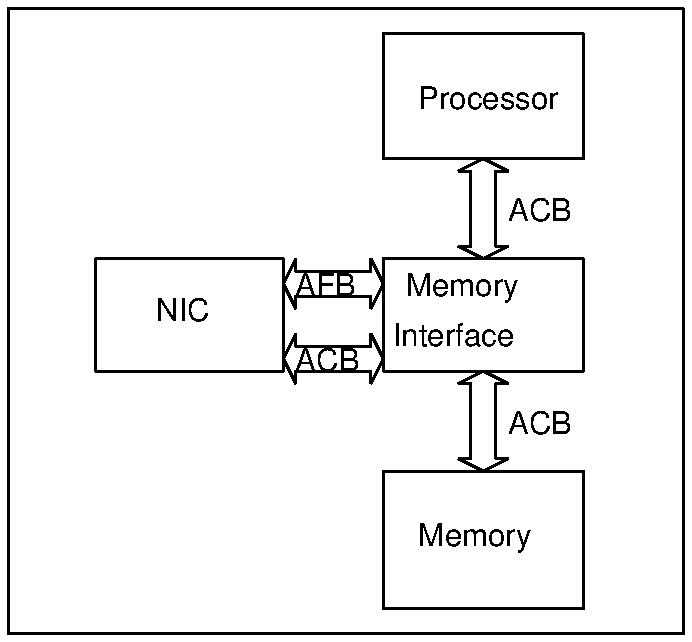
\includegraphics[width=8cm]{./figures/top_level.pdf}
			\caption{NIC, Processor and MEMORY interfaces}
			\label{fig:Interfaces}
		\end{figure}

	\begin{itemize}\label{ACB}
		\item ACB protocol : The NIC design includes two interfaces to support its functionality. The first interface is the ACB (AJIT Core Bus) interface, which enables the NIC to perform memory operations. Through the ACB interface, the NIC can receive Ethernet packets from the Xilinx's MAC IP and store them into the memory block assigned by the processor. It also allows the processor to access and process the stored packet data before transmission.
\newpage
		\begin{verbatim}
		1. Request packet:
		        A 110-bit format.
		        Request[109:0]
		        Request[109] = lock-bit
		        Request[108] = read/write-bar
		        Request[107:100] = byte mask
		                write data is organized as 8-bytes. 
		                if bit 7 (MSB) of byte-mask is set,
		                the top byte of write data is written, 
		                else not.
		        Request[99:64] = address (36-bit)
		        Request[63:0] = write-data.
		2. Response packet:
		        A 65-bit format.
		        Response[64] = Error
		        Response[63:0] = read-data
		3. For every request packet, there is a response.
		\end{verbatim}
	\end{itemize}

	

	\begin{itemize}\label{AFB}
		\item AFB protocol : The second interface is the AFB (AJIT FIFO Bus) interface, which is used by the processor to program the NIC registers and control its operation. The AFB interface enables the processor to start and stop the NIC, as well as provide the address of the interface data structure used for communication with the NIC.
		\begin{verbatim}
		1.  Request packet:
		        A 74-bit format,
		        Request[73:0]
		        Request[73]  = lock-bit
		        Request[72]  = read/write-bar 
		        Request[71:68] = byte mask
		                write data is organized as 4-bytes.
		                if bit 3 (MSb) of byte-massk is set,
		                the top byte of write data is written,
		                else not.
		        Request[67:32] = address (36-bit)
		        Request[31:0]  = write-data.
		2.  Response packet:
		        A 33-bit format,
		        Response[32] = Error
		        Response[31:0] = read-data
		\end{verbatim}
	\end{itemize}

By incorporating the NIC into the AJIT processor, the design enables efficient handling of incoming and outgoing Ethernet packets. The NIC supports the reception of Ethernet frames, parsing the necessary information such as MAC addresses and EtherType, and storing the payload data into the processor's assigned memory block. Similarly, it enables the processor to transmit Ethernet frames by retrieving the data from memory and encapsulating it into the appropriate Ethernet frame format.

With its ACB and AFB interfaces, the NIC provides a seamless interface between the AJIT processor and Ethernet networks, allowing for efficient communication and data exchange.


	\section{Interfaces data structures}

		The interface data structures used in the NIC design consist of three queues: the free\_queue, rx\_queue, and tx\_queue.



	\begin{itemize}
		\item \textbf{free\_queue}: This queue holds the addresses of free buffers that are available for storing packets. The processor initially assigns a set of buffers and pushes their addresses into the free\_queue. These buffers do not have any active packets and are ready to be utilized for storing incoming packets. Both the processor and the NIC can push and pop from the free\_queue.\\

		\item \textbf{rx\_queue}: The rx\_queue is pushed by the NIC and popped by the processor. It holds the addresses of buffers that currently contain active packets. When the NIC receives a packet, it stores the packet in a buffer and pushes the address of that buffer into the rx\_queue. This allows the processor to identify the buffers with active packets that are ready for processing.

		\item \textbf{tx\_queue}: The tx\_queue is pushed by the processor and popped by the NIC. Once the processor has finished processing a packet, it pushes the address of the processed packet buffer into the tx\_queue. The NIC monitors the tx\_queue and retrieves the buffer addresses from it to send the packets out over the network.\\
	\end{itemize}

These queues enable efficient coordination and communication between the processor and the NIC, ensuring the proper handling and processing of packets.The queue header format is shown below,
		\begin{verbatim}
		typedef struct _CortosQueueHeader {
		        uint32_t totalMsgs; // current total messages
		        uint32_t readIndex;
		        uint32_t writeIndex;
		        uint32_t length;
		        uint32_t msgSizeInBytes;
		        uint8_t *lock;
		        uint8_t *bget_addr;
		        // if misc == 1, then assume single writer 
		        // and single reader and don't use locks
		        uint32_t misc;
		} CortosQueueHeader;
		\end{verbatim}
	

To ensure synchronization and prevent conflicts during access to these queues, a locking mechanism is implemented. The locking mechanism utilizes atomic operations, which guarantee thread-safe access and modifications to the queues. This ensures that only one entity can perform push and pop operations on the queues at a given time, preventing simultaneous modifications and preserving the integrity of the queue data.


At startup, the processor initializes the queues by allocating memory for them and configuring their initial state. The addresses of these queues are then communicated to the NIC by writing to specific NIC registers. This process allows the NIC to access and manipulate the queues effectively during runtime. Let's see the NIC registers now.

	\section{NIC registers}

	The NIC (Network Interface Controller) registers are specific memory locations within the NIC that are used for configuration, control, and status monitoring purposes. These registers allow communication between the processor and the NIC, enabling the processor to control and monitor NIC. The NIC registers provide a standardized interface for the processor to interact with the NIC and perform tasks such as enabling or disabling the NIC, setting queue address and monitoring the status of data transmission and reception.

	\begin{table}[htbp]
		\centering
		\begin{tabular}{|c|c|c|}
			\hline
			Reg. ID& Address offset & Description  \\ \hline
			0  & 0x00  & Control reg    \\ \hline
			1  & 0x04  & Number of Servers    \\ \hline
			2  & 0x08  & Address of rx\_queue    \\ \hline
			10  & 0x28  & Address of tx\_queue    \\ \hline
			18  & 0x48  & Address of free queue    \\ \hline
		\end{tabular}
		\caption{NIC registers map}
		\label{tab:my_label1}
	\end{table}

	\newpage

	\section{NIC Architecture}
The NIC is designed to handle the reception and transmission of Ethernet packets. It utilizes different daemons, each serving a specific purpose, to perform the necessary operations. These daemons work collaboratively to ensure the smooth flow of data between the processor and the network interface.


		\begin{figure}[htbp!]
			\centering
			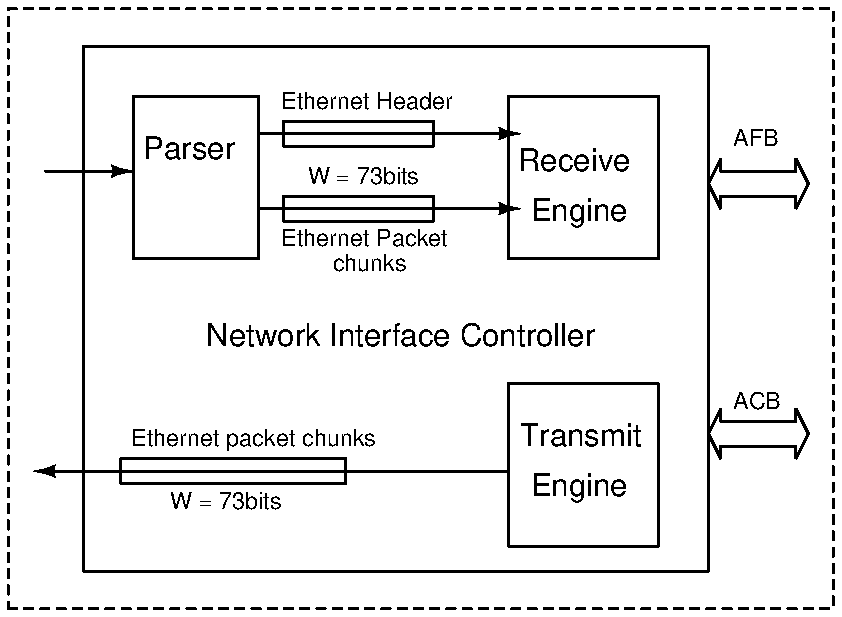
\includegraphics[width=12cm]{./figures/NIC_arch.pdf}
			\caption{NIC architecture}
			\label{fig:NIC}
		\end{figure}

	NIC reads 73 bit data chunks from MAC and sends it to parser deamon, the 73 bits are splitted as follows,
	\begin{table}[htbp]
		\centering
		\begin{tabular}{|c|c|c|}
			\hline
			tlast&tdata &tkeep  \\ \hline
			1 bit  &64 bits  & 8 bits    \\ \hline
		\end{tabular}
		\caption{Input packet chunk from MAC}
		\label{tab:NIC_input_output}
	\end{table}


	\begin{enumerate}
		\item \textbf{Parser Daemon}: The parser daemon, receives data from the MAC (Media Access Control) through a pipe and extracts relevant information from Ethernet packets. It utilizes a state machine to process chunks of data and identifies essential details such as source and destination MAC addresses, type/length field, and packet data. The parsed information is then forwarded to receve engine daemon.
		\begin{verbatim}
			loop1 :
			if(enable_by_processor)
			       loop2 :
			       -> read from MAC
			       -> if(Header) 
			                -> send to header & packet pipe
			                -> goto loop2
			       -> else
			       	        -> send to packet pipe
			       	        -> goto loop2
			else
			       -> goto loop1
		\end{verbatim}

		\item \textbf{Receive Engine Daemon}: The receive engine daemon is responsible for storage of packets coming from parser. It receives the parsed packet information from the parser daemon and interacts with the processor to ensure the proper handling of received packets. The receive engine daemon uses the free\_queue, to get empty buffer address tp store the active packets in buffers.
			Then uses rx\_queue to provide their(buffer's) addresses to the processor for processing. The algorith of receive engine is shown below,
		\begin{verbatim}
			loop1 :
			if(enable_by_processor)
			       loop2 :
			       -> count = 0;
			       -> buf_addr = pop from free queue
			       loop2.1:
			       -> Read from header_pipe and write to buff_addr
			       -> count++
			       -> if(!header_end)
			       	        -> goto loop2.1
			       loop2.2:
			       -> Read from packet pipe and write to buf_addr 
			       -> count++
			       -> if(last_chunk)
			       	        -> write count and last bytemast to buf_addr[0].
			       	        -> push buf_addr to rx_queue.
			                -> goto loop2
			       -> else
			       	        -> goto loop2.2
			else
			       -> goto loop1
		\end{verbatim}

		\item \textbf{Transmit Engine Daemon}: The transmit engine daemon focuses on transmitting processed packets from the processor to the external network. It receives the addresses of processed packet buffers from the processor via the tx\_queue and sends the corresponding packets out through the Ethernet interface. The transmit engine daemon monitors the tx\_queue and retrieves the buffer addresses to facilitate efficient packet transmission. The daemon also pushes free\_queue with the address of buffer which is sent out. This allows resue of buffers. The algorith of transmit engine is shown below,
		\begin{verbatim}
			loop1 : 
			if(enable_by_processor)
			        loop2:
			        -> buf_addr = try to pop tx_queue
			        -> if(pop successful)
			                -> Rx = read control data(buf_addr[0]) 
			                -> count = extractCountFromRx(Rx)
			                loop3:
			                -> read packet from buf_addr
			                -> send out to MAC
			                -> count--
			                -> if(count == 0)
			                        -> push buf_addr to free_queue.
			                        -> goto loop2 
			                -> else
			                        -> goto loop3
			        -> else
			                        -> goto loop2
			->else
			        goto loop1
		\end{verbatim}

	\item \textbf{Software Register Access Daemon}: The software register access daemon enables the processor to access and modify the NIC's software registers. These registers contain various control and configuration parameters, allowing the processor to configure and manage the behavior of the NIC. The software register access daemon handles the communication between the processor and the NIC registers, ensuring reliable and secure access. Processor uses AFB protocol(see ~\ref{AFB}) for register access.\\

		\item \textbf{NIC Register Access Daemon}: The NIC register access daemon provides the necessary interface for the NIC to read from and write to its internal registers. These registers store critical information for the proper functioning of the NIC, including configuration settings, status flags, and other control parameters. The NIC register access daemon ensures that the processor can interact with these registers and modify them as needed to configure and manage the NIC's behavior.\\
	\begin{itemize}
		\item NIC Register Access Protocol :
		\begin{verbatim}
		1.  Request packet:
		        A 43-bit format,
		        Request[42]  = rwbar
		        Request[41 : 38]  = bmask 
	        	Request[37 : 32] = index
		        Request[31:0]  = write-data
		2.  Response packet:
		        A 33-bit format,
		        Response[32] = Response Status
		        Response[31:0] = response-data
		\end{verbatim}
	\end{itemize}

	\end{enumerate}

Together, these daemons form an integral part of the NIC design, enabling the integration of Ethernet functionality into the AJIT processor. They work in collaboration to handle packet reception, processing, and transmission, ensuring efficient communication between the processor and the network.


				%\end{itemize}


	\section{Validation and Performance}
	
	The data rate found using 1x1x32 (single core single threaded) AJIT processor are as shown in table~\ref{table_dataRate}
	\begin{table*}[h!]
		\caption{Data rate achieved for differnet number of packets \& packet sizes}
		\begin{center}
			\begin{tabular}{|c|c|c|c|}
				\hline
				& \multicolumn{3}{c|}{\textbf{Packet Size}(in Bytes)}\\
				\hline
				\textbf{No. of Packets}& \textbf{48}			& \textbf{136}			& \textbf{236} 	  \\
				\hline
				&  \multicolumn{3}{c|}{\textbf{Data Rate}(in Mbps)}\\	
				\hline
				1			& 11.3316		  	& 31.7085			& 51.2869 \\
				\hline
				10			& 18.8431		  	& 57.2255			& 102.4069\\
				\hline
				100			& 22.4589		  	& 64.1140			& 110.9845\\
				\hline
				500			& 22.9792		  	& 64.0819			& 114.2853\\
				\hline
				1000			& 23.0982			& 64.0665			& 114.4293\\
				\hline
				5000			& 23.0336			& 64.3663			& 114.7432\\
				\hline
				10000			& 23.0892			& 64.3163			& 114.7907\\
				\hline
				50000			& 23.0983			& 64.4662			& 114.8123\\
				\hline
			\end{tabular}
			\label{table_dataRate}
		\end{center}
	\end{table*}
	
	Only NIC with Memory we are able to achieve 433.2847 Mbps for 1750 packets of size 146 Byets.


\chapter{Integrating Xilinx MAC IP}

	\section{Options Considered}
	\section{100Mbps MAC on KC705 and VCU128 FPGA}
	\section{10Gbps MAC on VC709 FPGA}

\chapter{SOC design and validation}
	\section{Processor with NIC and MAC}
	\section{Processor with NIC, MAC and Acclerator}

		\begin{figure}[h]
			\centering
			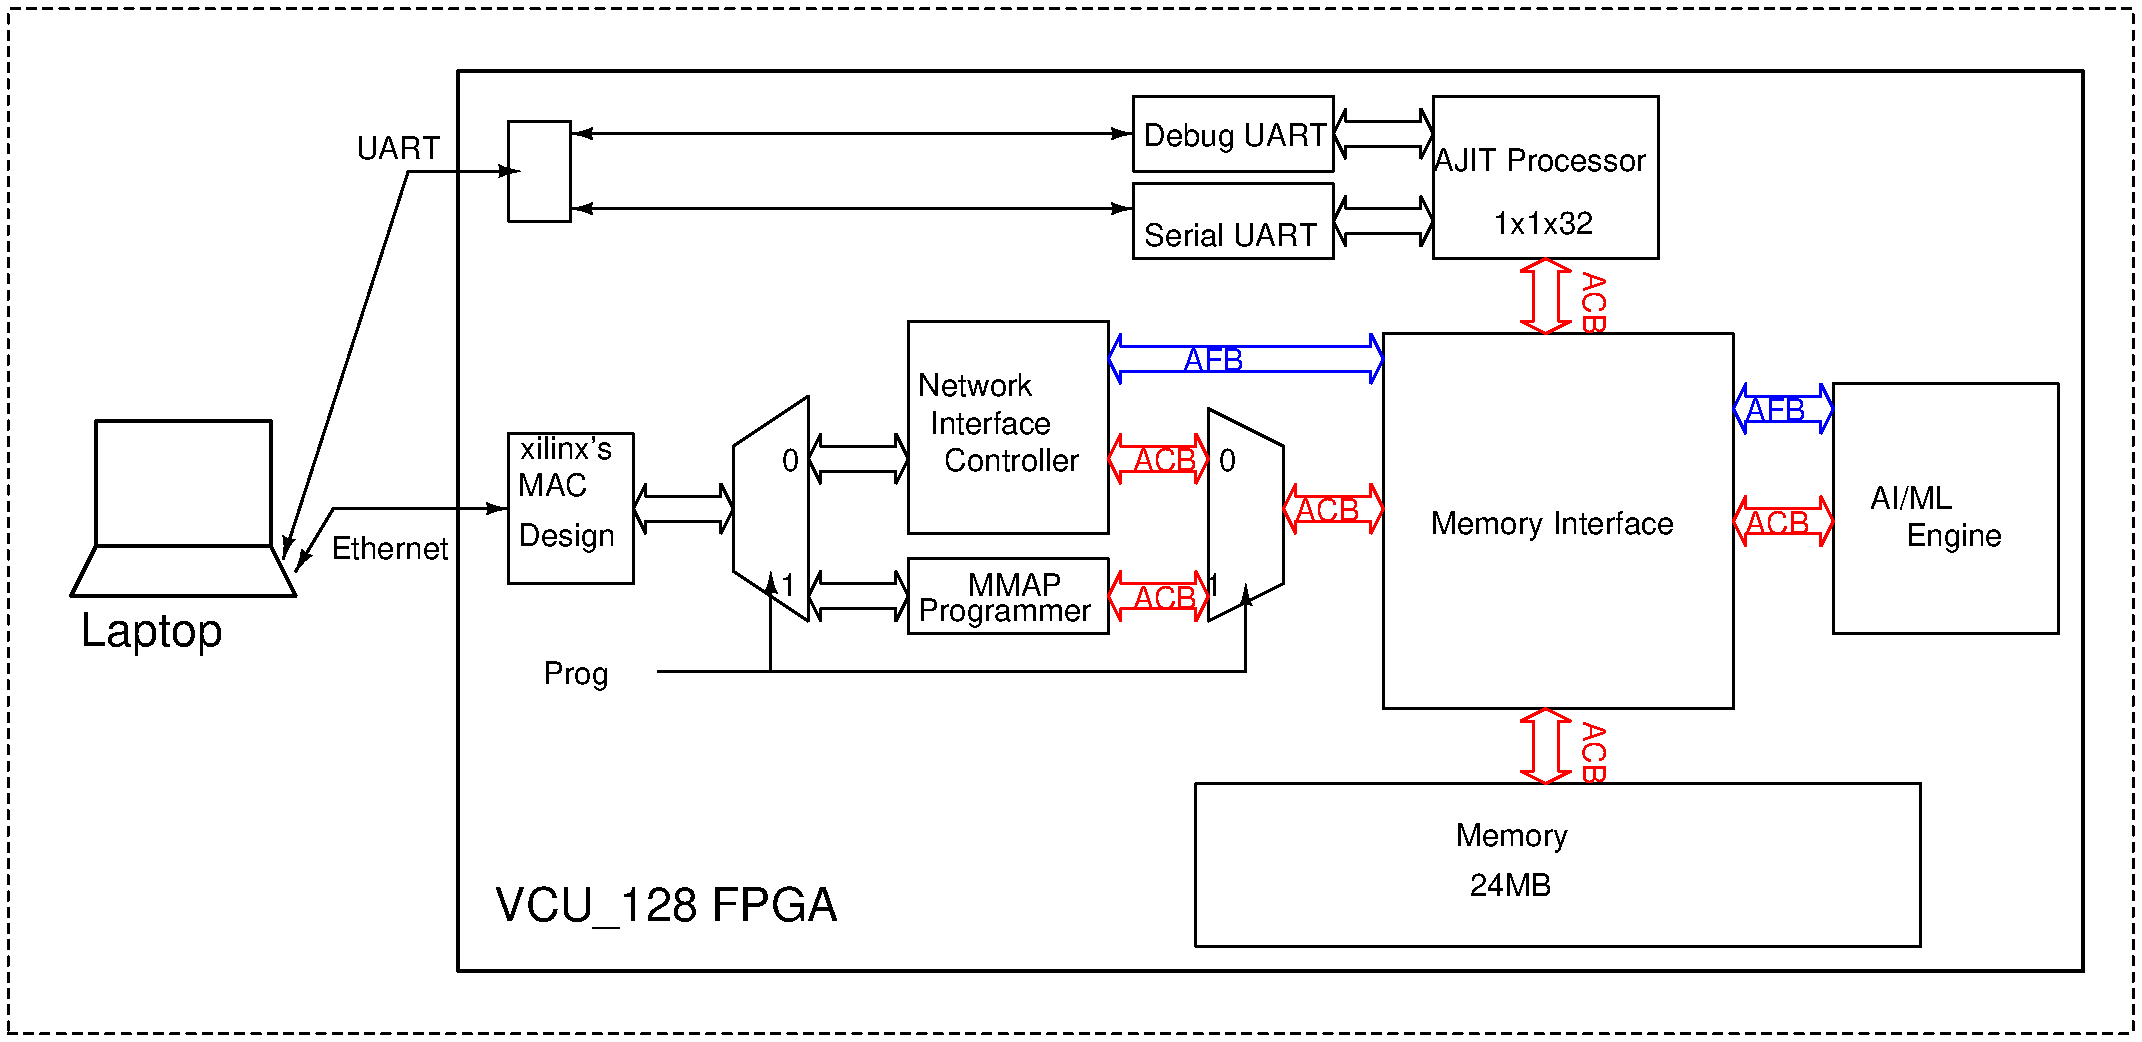
\includegraphics[width=14cm]{./figures/NIC_MAC_ACCL_PROC.pdf}
			\caption{system with accelerator and netwrok interface}
			\label{fig:SystemACCL}
		\end{figure}



	\section{Boot sequence}

\chapter{Summary and Conclusions}
\end{comment}

	\begin{comment}
	\subsubsection{MAC-NIC Inteface}
	The MAC is connected to two FIFOs on the host side namely the Tx\_FIFO and the Rx\_FIFO. The Rx\_FIFO is responsible for 
	the buffering of data sent from the MAC so that the NIC can access the packet at a slightly leisurely pace. The Tx\_FIFO buffers the 
	packet to be transmitted by the MAC until the MAC is ready to transmit. The communication between the NIC and the FIFO occurs via the 
	AHIR pipe protocol. The pipe here is defined to be a 73-bit wide pipe, that consists of all the data sent by the MAC on 
	the AXI-s side of the interface or alternatively all the data to be sent to the MAC by the host. \\
	The format of the 73-bit data quantity on the pipe is as follows : 
	

	\textbf{Error Detection}: The MAC does not discard the erroneous packets but instead asserts a signal (tuser) while transmitting the last 
	word of a bad packet. The RX\_FIFO notifies the MAC that a bad packet has been received via the 73-bit data word defined earlier, 
	consisting of a unique data pattern (which identifies a bad packet):
	
	\begin{table}[htbp]
		\centering
		\begin{tabular}{|c|c|c|}
			\hline
			tlast&tdata &tkeep  \\ \hline
			`0'   &0xFFFFFFFFFFFFFFFF  & 0x00    \\ \hline
			
		\end{tabular}
		\caption{Error chunk format}
		\label{tab:my_label1}
	\end{table}

	When the NIC receives this bad packet identifier, it does not set the flag buffer bit (defined later) and therefore 
	the bad packet is not processed by the host.    
	\end{comment}

	

\end{document}
